\documentclass[11pt,a4paper]{article}

% ---------- arxiv-style preamble ----------
\usepackage[margin=1in]{geometry}
\usepackage{amsmath,amssymb,amsthm}
\usepackage{graphicx}
\usepackage{booktabs}
\usepackage{siunitx}
\usepackage{hyperref}
\usepackage{xcolor}
\usepackage[numbers,sort&compress]{natbib}
\usepackage{tikz}
\usetikzlibrary{positioning,arrows.meta,matrix}
\usepackage{pgfplots}
\pgfplotsset{compat=1.18}
\usepackage{caption}
\usepackage{listings}
\usepackage{array}
\captionsetup{font=small,labelfont=bf}
\hypersetup{
  colorlinks=true,
  linkcolor=blue!50!black,
  citecolor=blue!50!black,
  urlcolor=blue!50!black
}

\providecommand{\tierBlue}{\textbf{[BLUE]}}
\providecommand{\tierGreen}{\textbf{[GREEN]}}
\providecommand{\tierYellow}{\textbf{[YELLOW]}}
\providecommand{\tierOrange}{\textbf{[ORANGE]}}
\providecommand{\tierRed}{\textbf{[RED]}}

\title{
  \textbf{Collective $\Phi$ Axis-Orthogonality: hivemind integration is mediated by PID synergy and $\partial\Phi/\partial I$, not by Kuramoto sync, pair polarity, or bivariate transfer entropy}\\[4pt]
  \large An 8-cell hexa-native verify raster across axis F (HIVE-MIND) rounds 1--3
}

\author{
  \texttt{anima} maintainers\\
  \normalsize\textit{dancinlab}\\[2pt]
  \normalsize\href{https://github.com/dancinlab/anima}{\texttt{github.com/dancinlab/anima}}
}

\date{\today}

\begin{document}

\maketitle

% =========================================================================
\begin{abstract}
We ran eight pre-registered, deterministic, hexa-native measurements
(\texttt{UNIVERSE/H\_354,355,609--611,617--619}) that probe whether
\emph{collective big-$\Phi$} -- the cause-effect Integrated
Information Theory (IIT) 4.0 quantity computed on a two-substrate
``hivemind'' system $A \otimes_W B$ -- aligns with the four most
common dynamical proxies for inter-substrate coupling:
(i)~Kuramoto-style phase synchronisation time
($\tau_{\mathrm{sync}}$ vs $\tau_{\mathrm{cons}}$),
(ii)~pair polarity (attractive / repulsive / bipolar coupling
sign), (iii)~bivariate transfer entropy ($\mathrm{TE}_{A \to B}$),
and (iv)~3-source PID synergy / $\partial\Phi/\partial I$.
Three of the four proxy axes (i--iii) close
\tierRed\ \emph{closed-negative}: Pearson
$|r|<0.32$ against collective $\Phi$, with
spread-to-floor ratios $\geq 13\times$ and pre-registered
falsifiers FAILing in every case. Two further channels
close \tierGreen\ \emph{supported}:
(v)~PID synergy ratio
($\mathrm{ratio}=1.0$ across $K \in \{0, \tfrac13, \tfrac23, 1\}$,
H\_355) and (vi)~$\partial\Phi_{\mathrm{coll}}/\partial I$ peak
location at $I = \mathrm{GZ\_LOWER}=0.21$ with
$|\Delta|=0.002$ ($21\times$ margin, H\_618). A SAVANT$\times$HIVE
cross-link round-3 closes the dissociation: single-substrate
SAVANT inhibition produces a hivemind PID synergy
\emph{monotone-decay} signature (H\_619, $7/7$ falsifiers PASS) but
yields $SI_{\mathrm{collective}}=1.005 \ll 3$, $21\times$ below
the H\_348 threshold (H\_617). The combined raster therefore
identifies the real collective-$\Phi$ axis as
\emph{higher-order information-integration} (PID synergy +
$\partial\Phi/\partial I$ susceptibility), not pairwise
dynamics. This is a negative-result arc:
five out of eight cells are closed-negative, and the value
of the paper is the dissociation matrix it pins down
\citep{anima_g73}.
\end{abstract}

\section{Introduction}
\label{sec:intro}

The combination problem of consciousness asks how separate phenomenal
substrates compose into a single integrated experience
\citep{tononi2016iit,oizumi2014phenomenology,albantakis2023iit4}. In
Integrated Information Theory (IIT) 4.0, the natural composition
quantity is the \emph{collective} cause-effect $\Phi$ of a joint system
$A \otimes_W B$, where $W \in [0,1]$ parameterises cross-substrate
coupling. Two questions arise. \emph{First}, what dynamical observable
on the joint state tracks collective $\Phi$? \emph{Second}, when an
observable does \emph{not} track collective $\Phi$, is the
observable failing to measure integration, or is collective $\Phi$
itself orthogonal to that observable's natural axis?

The previously catalogued single-substrate result is that bivariate
transfer entropy (TE), bivariate Pearson correlation, and Shannon
entropy of the state-visit distribution are all closed-negative
against single-substrate $\Phi$
\citep{anima_H207,anima_H290}, while net 3-source PID synergy and the
derivative $\partial\Phi/\partial I$ (where $I$ is an inhibition
modulator) track it strongly
\citep{anima_H293,anima_H294}. The natural pre-registered hypothesis
is that the same axis-orthogonality pattern repeats on the
\emph{collective} side. We tested this in three rounds, eight
hypothesis cells, across axis F (HIVE-MIND) of the public
\texttt{anima} hypothesis ledger.

\medskip
\noindent\textbf{Contributions.}
\begin{enumerate}\itemsep0.3em
\item \emph{Round 1 closed-negative trilogy.}
      Kuramoto $\tau_{\mathrm{sync}}$ vs $\tau_{\mathrm{cons}}$
      (H\_354, $r=0.04$, spread $45\times$, \tierRed),
      pair polarity ANOVA across attract / repel / bipolar
      coupling (H\_610, $F=0.36$, spread/std $=0.41$, \tierRed),
      and bivariate transfer entropy on a 6-rule $\times$ 4-W
      panel (H\_611, $r=0.31$ vs the H\_290 anchor $r=0.883$, \tierRed).
\item \emph{Round 1--2 PID/$\partial\Phi/\partial I$ supports.}
      Net 3-source PID synergy ratio is $1.0$ across all
      non-degenerate $K$ buckets on an XOR-family hivemind
      (H\_355, \tierGreen), super-additivity is observed at
      $(110, 110, W{=}0.6)$ with $\Delta = +10.48$ (H\_609,
      \tierGreen), and the $\partial\Phi_{\mathrm{coll}}/\partial I$
      peak lands at $I = \mathrm{GZ\_LOWER}=0.21$ with a $|\Delta|=0.002$
      margin ($21\times$ tighter than the pre-registered $0.05$
      tolerance, H\_618, \tierGreen).
\item \emph{Round 3 cross-link dissociation.}
      SAVANT-inhibition modulates hivemind PID synergy in a
      monotone-decay pattern (H\_619, $7/7$ falsifiers PASS,
      \tierGreen), yet the same inhibition produces
      $SI_{\mathrm{collective}}=1.005$ at $\mathrm{GZ\_LOWER}$
      ($21\times$ below the pre-registered $SI > 3$ floor,
      H\_617, \tierRed). Substrate-isolation in the single-substrate
      saga therefore does \emph{not} carry over to collective
      integration; the cross-link is axis-orthogonal.
\item All eight measurements are deterministic and hexa-native;
      each cell ships a \texttt{run.hexa} source file, a
      \texttt{run.log} verbatim transcript, and a
      \texttt{result.json} machine-readable verdict on the public
      \texttt{anima} main branch under anti-fake-closure governance
      \citep{anima_g73}.
\end{enumerate}

\medskip
\noindent\textbf{Negative-result framing.}
Five of the eight cells close \tierRed\ closed-negative. We do not
treat this as a setback. Following \texttt{a\_paper\_negative\_ok}
governance (\S\ref{sec:repro}), a closed-negative result that
deterministically rules out an axis is a valid finding. The paper's
contribution is precisely the dissociation matrix
(\S\ref{sec:dissoc}, Fig.~\ref{fig:dissoc}): collective $\Phi$ is
co-axial with PID synergy and $\partial\Phi/\partial I$, and
axis-orthogonal to Kuramoto $\tau$, pair polarity, and bivariate
TE.

\section{Background}
\label{sec:bg}

\subsection{Hivemind substrate $A \otimes_W B$}
\label{sec:hivemind-substrate}

A hivemind substrate is a pair $(A, B)$ of binary cellular automata
with their own transition rules $r_A, r_B$ and local cell counts
$n_A, n_B$, composed into a joint $n_A + n_B$-cell system whose
transition probability matrix (TPM) is
\[
  \mathrm{TPM}_{AB}(s, s')
  = (1-W) \cdot \mathrm{TPM}_A^{\mathrm{own}}(s, s') \,\cdot\,
    \mathrm{TPM}_B^{\mathrm{own}}(s, s')
    + W \cdot \mathrm{TPM}^{\mathrm{cross}}(s, s'),
\]
where $W \in [0,1]$ is the coupling weight. Setting $W=0$ recovers two
independent substrates (a sanity-check ``decoupled anchor''); setting
$W=1$ replaces the own-dynamics by a cross-substrate XOR/blend rule.
The collective big-$\Phi$ is the IIT 4.0 cause-effect $\Phi$ of the
joint $n_A + n_B$-cell substrate at a chosen system state, computed via
\texttt{HEXAD/IIT4/lib/big\_phi.hexa} with bounded purview cap (typically
$\mathrm{cap}_{n=6}=2$, the M4b SSOT).

\subsection{Four proxy axes}

The four proxy axes tested by this paper are the standard dynamical
observables an experimenter is most likely to substitute for
collective $\Phi$.

\paragraph{Kuramoto synchronisation time.}
For each substrate $s_i$ we attach a phase $\theta_i(t)$ with
intrinsic frequency $\omega_i \sim \mathcal{N}(0, 1)$. The standard
Kuramoto model \citep{kuramoto1984chemical,acebron2005kuramoto}
\[
  \dot \theta_i = \omega_i + \frac{K}{n}\sum_{j} \sin(\theta_j - \theta_i)
\]
yields a sync time $\tau_{\mathrm{sync}}$ at which the order parameter
$r = |\frac{1}{n}\sum_j e^{i\theta_j}| > 0.9$. We compare this with
the consensus time $\tau_{\mathrm{cons}}$ for blend-to-mean
convergence in the substrate state space, a closed-form proxy
mathematically equivalent to the H\_352 \texttt{hive\_state\_sync}
module.

\paragraph{Pair polarity.}
A coupling polarity $\pi \in \{\text{attract}, \text{repel}, \text{bipolar}\}$
biases the cross-substrate XOR/blend rule by an additive
$\pm \delta$ in the next-state probability. The natural intuition
is that attractive coupling should drive higher collective $\Phi$
than repulsive coupling. We test this with a between-polarity ANOVA
on the collective $\Phi$ measurements.

\paragraph{Bivariate transfer entropy.}
Schreiber's TE \citep{schreiber2000te} is the most-deployed
information-theoretic measure of directed information flow between
two substrates,
\[
  \mathrm{TE}_{A \to B} =
  \sum p(b_{t+1}, b_t^{(k)}, a_t^{(\ell)}) \log
  \frac{p(b_{t+1} \mid b_t^{(k)}, a_t^{(\ell)})}{p(b_{t+1} \mid b_t^{(k)})}.
\]
We compute it on the deterministic two-substrate ECA panel with
$n_A = n_B = 2$.

\paragraph{Net 3-source PID synergy.}
We use the McGill 3-variate co-information
\citep{mcgill1954multivariate} (signed: $> 0 \Rightarrow$ synergy,
$< 0 \Rightarrow$ redundancy) as a closed-form summary of the
Williams-Beer PID lattice \citep{williams2010pid,bertschinger2014synergistic}.
Specifically
\[
  \mathrm{II}_3(T; S_0, S_1, S_2)
  = \sum_i I(T; S_i) - \sum_{i<j} I(T; S_i, S_j)
    + I(T; S_0, S_1, S_2),
\]
and the synergy ratio $\mathrm{ratio} =
\mathrm{II}_3 / (\mathrm{II}_3 + R_{\mathrm{red}})$ uses the
identity-cell anchor.

\subsection{Anti-fake-closure governance}
\label{sec:antifake}

A verdict is \emph{earned} by an independent deterministic recompute
that could have falsified the claim; a function arranged to return
the value it is then compared against is a tautology, not a
verification \citep{anima_g73}. All eight cells in this paper carry
pre-registered falsifiers ($n=5$--$7$ per cell, $44$ total) and
PASS/FAIL outcomes against pre-registered thresholds. The verbatim
verdicts are reproduced in \S\ref{sec:verify} and are stored on
the public \texttt{anima} main branch.

% =========================================================================
\section{Method}
\label{sec:method}

\subsection{Cell roster}
\label{sec:roster}

Table~\ref{tab:roster} summarises the eight cells, the proxy axis each
probes, and the pre-registered falsifier count. Three cells (H\_354,
H\_610, H\_611) probe pairwise dynamical observables on the joint
state, three cells (H\_355, H\_609, H\_618) probe higher-order
information-integration observables, and two cells (H\_619, H\_617)
test the SAVANT$\times$HIVE cross-link in round 3.

\begin{table}[h]
\centering
\small
\begin{tabular}{lllll}
\toprule
\textbf{H\_id} & \textbf{axis} & \textbf{round} &
\textbf{proxy probed} & \textbf{PR} \\
\midrule
H\_354 & F1 & 1 & Kuramoto $\tau_{\mathrm{sync}}$ vs $\tau_{\mathrm{cons}}$ & \#1156 \\
H\_355 & F1 & 1 & net 3-source PID synergy on hivemind XOR & \#1160 \\
H\_609 & F1 & 2 & super-additivity $\Phi(AB) > \Phi(A) + \Phi(B)$ & \#1168 \\
H\_610 & F1 & 2 & pair polarity (attract / repel / bipolar) ANOVA & \#1164 \\
H\_611 & F1 & 2 & bivariate transfer entropy on 6-rule $\times$ 4-W panel & \#1163 \\
H\_617 & E$\times$F & 3 & SAVANT$\times$HIVE SI\_collective & \#1171 \\
H\_618 & E$\times$F & 3 & $\partial\Phi_{\mathrm{coll}} / \partial I$ peak location & \#1175 \\
H\_619 & E$\times$F & 3 & PID synergy under SAVANT inhibition $I$ & \#1172 \\
\bottomrule
\end{tabular}
\caption{Eight-cell roster for the collective-$\Phi$ axis-orthogonality
raster. Rounds 1 and 2 probe pairwise vs higher-order observables on
the same homogeneous-rule hivemind family; round 3 introduces the
SAVANT inhibition modulator from axis E to test cross-link
dissociation.}
\label{tab:roster}
\end{table}

\subsection{Cell parameters}

For Kuramoto (H\_354) we sweep $n_{\mathrm{sub}} \in \{3,5,7\}$ and
$K \in \{0.5, 1.0, 2.0, 3.0\}$, $\mathrm{dt}=0.05$, sync threshold
$r > 0.9$, consensus threshold $\|s - \bar s\| < 0.05$, 12 cells.
PID (H\_355) sweeps a length-3 mask over $K \in \{0,
\tfrac{1}{3}, \tfrac{2}{3}, 1\}$, 8 permutations.
Super-additivity (H\_609) sweeps 5 rule pairs $\times$ 4 $W$
values, $\mathrm{cap}_{n=3}=3$, $\mathrm{cap}_{n=6}=2$.
Pair polarity (H\_610) sweeps 3 polarities $\times$ 3 $W$ values
$\times$ 3 rule pairs $\times$ 3 system states (reduced from $n=4$),
9 measurements per polarity. Bivariate TE (H\_611) sweeps 6 rules
$\times$ 4 $W$ values, $n_A = n_B = 2$. Round-3 cells (H\_617--619)
fix the focal $(110, 110, W{=}0.6)$ point and sweep inhibition
$I \in [0.05, 0.5]$ with the SAVANT focal $\mathrm{GZ\_LOWER}
= \tfrac{1}{2} - \ln(\tfrac{4}{3}) = 0.21232$
\citep{anima_H348}.

\subsection{Falsifiers and pre-registered thresholds}

Each cell carries 5--7 pre-registered falsifiers. Examples:
\begin{itemize}\itemsep0.2em
\item H\_354: $\mathrm{C1}: |r(\tau_{\mathrm{sync}},
      \tau_{\mathrm{cons}})| > 0.5$;
      $\mathrm{C2}: \mathrm{spread} = \tau_{\mathrm{cons}}/\tau_{\mathrm{sync}}
      \leq 2$.
      Verdict rule: FALSIFIED iff $|r| < 0.3 \wedge \mathrm{spread} > 5$.
\item H\_355: synergy ratio $> 0.5$ on the non-trivial mask mean;
      strict monotone increase of synergy in $K$.
\item H\_609: super-additivity floor $\Delta_{\max} > 0$;
      $W$-monotone $\Delta(W=0) < \Delta(W=0.3) < \Delta(W=0.6) < \Delta(W=1.0)$.
\item H\_610: between-polarity ANOVA $F > F_{\mathrm{crit}}^{\alpha=0.05}$ and
      $\mathrm{spread}/\mathrm{std} > 1$.
\item H\_611: Pearson $r(\Phi_{\mathrm{coll}}, \mathrm{TE}_{A\to B}) > 0.5$.
\item H\_617: $SI_{\mathrm{collective}}(\mathrm{GZ\_LOWER}) > 3$ and
      monotone decrease across the $I$ sweep.
\item H\_618: $|\Delta_{\mathrm{argpeak}}| \leq 0.05$ for the
      $\partial\Phi_{\mathrm{coll}}/\partial I$ peak location.
\item H\_619: synergy-ratio spread $\geq 0.05$ across the $I$ sweep
      \emph{and} monotone-decay constraint (at most 1 inversion).
\end{itemize}

\subsection{Compute envelope}

All eight cells ran $\$0$ Mac-local foreground in
\texttt{hexa run} mode, total wall time $\sim 6$ minutes; the
longest single cell was H\_611 ($\sim 180$ s) for the 6-rule
$\times$ 4-W TE panel. No GPU. Cells are byte-identical across
re-runs on the same machine; cross-machine reproducibility is
checked by the determinism falsifier in each cell.

% =========================================================================
\section{Round 1 + 2: the closed-negative trilogy on pairwise observables}
\label{sec:closed-neg}

\subsection{H\_354 -- Kuramoto sync $\tau_{\mathrm{sync}}$ does not predict consensus $\tau_{\mathrm{cons}}$}
\label{sec:h354}

Table~\ref{tab:h354} reports the 12-cell sweep. Pearson
$r(\tau_{\mathrm{sync}}, \tau_{\mathrm{cons}}) = 0.04$, more than
$12\times$ below the pre-registered $> 0.5$ floor. The ratio
$\tau_{\mathrm{cons}}/\tau_{\mathrm{sync}}$ spans
$[0.016, 0.722]$, a $45\times$ spread, more than $20\times$ above the
$\leq 2$ falsifier ceiling. The two clocks are decoupled: phase
synchronisation does not predict substrate-state consensus.

\begin{table}[h]
\centering
\small
\begin{tabular}{rrrrrr}
\toprule
\textbf{$n$} & \textbf{$K$} & \textbf{$\tau_{\mathrm{sync}}$}
& \textbf{$\tau_{\mathrm{cons}}$}
& \textbf{ratio $\tau_{\mathrm{cons}}/\tau_{\mathrm{sync}}$} & \\
\midrule
3 & 0.5 &  115 & 83 & 0.722 & \\
3 & 1.0 &  478 & 41 & 0.086 & \\
3 & 2.0 &   48 & 19 & 0.396 & \\
3 & 3.0 &   35 & 12 & 0.343 & \\
5 & 0.5 &  450 & 82 & 0.182 & \\
5 & 1.0 &  154 & 40 & 0.260 & \\
5 & 2.0 & 1200 & 19 & 0.016 & (cap) \\
5 & 3.0 &  106 & 12 & 0.113 & \\
7 & 0.5 &  657 & 83 & 0.126 & \\
7 & 1.0 & 1200 & 41 & 0.034 & (cap) \\
7 & 2.0 & 1200 & 20 & 0.017 & (cap) \\
7 & 3.0 &   32 & 12 & 0.375 & \\
\midrule
\multicolumn{4}{l}{\textbf{Pearson $r = 0.041$ ($\ll 0.5$ floor)}} & & \\
\multicolumn{4}{l}{\textbf{spread $= 45.6\times$ ($\gg 2.0$ ceiling)}} & & \\
\multicolumn{4}{l}{\textbf{Verdict: \tierRed\ FALSIFIED (4/5 falsifiers FAIL)}} & & \\
\bottomrule
\end{tabular}
\caption{H\_354 Kuramoto sweep. Two clocks (phase $\tau_{\mathrm{sync}}$
vs substrate-state $\tau_{\mathrm{cons}}$) are decoupled; the
$45\times$ ratio spread is dominated by the high-$n$ low-$K$ cap of
1200 vs the fast consensus floor of $\sim 20$ steps.}
\label{tab:h354}
\end{table}

\subsection{H\_610 -- pair polarity does not separate collective $\Phi$}
\label{sec:h610}

A 27-measurement sweep over polarity $\in \{\text{attract},
\text{repel}, \text{bipolar}\}$, $W \in \{0.3, 0.5, 0.8\}$, and rule
pairs $\{(110,110), (30,30), (110,30)\}$. The between-polarity
means are
$\bar\Phi_{\mathrm{attract}} = 4.30$,
$\bar\Phi_{\mathrm{repel}} = 2.25$,
$\bar\Phi_{\mathrm{bipolar}} = 2.98$,
with pooled $\sigma = 4.97$ and ANOVA $F = 0.36$
(df $= 2/24$, $F_{\mathrm{crit}}^{\alpha=0.05} = 3.40$).
The spread-to-pooled-std ratio is $0.41$, well below 1; the
polarity factor does not separate the collective-$\Phi$ samples,
and the closed-form ANOVA also fails.

\subsection{H\_611 -- bivariate transfer entropy is XOR-blind}
\label{sec:h611}

A 24-measurement sweep over 6 rules $\times$ 4 $W$ values gives
Pearson $r(\Phi_{\mathrm{coll}}, \mathrm{TE}_{A\to B}) = 0.31$,
Spearman $\rho = 0.26$. The H\_290 single-substrate anchor for the
same family is $r = 0.883$ \citep{anima_H290}, so the collective
side under-aligns by a factor of $0.31/0.883 = 0.35$. The cause is
diagnostic: bivariate TE is \emph{XOR-blind} on the rules 30, 90,
105, 150 in the panel (TE$_{A\to B}=0$ whenever the cross-rule has
even parity in cell flips), while $\Phi_{\mathrm{coll}}$ is
non-zero for those same rules at $W \in \{0.6, 1.0\}$
(see panel data in \S\ref{sec:verify}). H\_611 is therefore
\tierRed\ FALSIFIED, and the reason is structural rather than noise.

\subsection{Cross-row pattern: pairwise observables do not see higher-order integration}

The three closed-negative cells share a feature: each measures a
pairwise dynamical observable -- Kuramoto phase-locking
($\theta_i - \theta_j$), polarity-weighted next-state bias
($\pm \delta$), bivariate transfer entropy ($A \to B$ only). The
joint substrate's cause-effect $\Phi$ is the
union of \emph{all} subset purviews, including 3- and
4-cell synergistic purviews, so it is not a function of any
fixed-order pairwise quantity. The closed-negative trilogy is
internally consistent.

% =========================================================================
\section{Round 1 + 2: PID synergy and $\partial\Phi/\partial I$ supports}
\label{sec:supports}

\subsection{H\_355 -- net PID synergy is constant 1.0 across $K$}

On the 3 binary substrates $\times$ 1 cell hivemind, the 8-permutation
net 3-source PID gives synergy $\in \{0, 1, 2, 3\}$ (mask-weight
linear), redundancy $= 0$, and synergy ratio $= 1.0$ across all
non-degenerate $K$-buckets (Table~\ref{tab:h355}). The XOR-family
substrate is intrinsically synergy-pure; the result anchors the
hivemind PID against the sister single-substrate
H\_293/H\_294 saga \citep{anima_H293,anima_H294}, where the same
sign-convention gives a strong $\Phi$-tracking signal. Five of five
falsifiers PASS. \tierGreen\ SUPPORTED.

\begin{table}[h]
\centering
\small
\begin{tabular}{rcccc}
\toprule
\textbf{$K$} & \textbf{$\overline{\text{synergy}}$} &
\textbf{$\overline{\text{redundancy}}$} &
\textbf{$\overline{\text{ratio}}$} & \textbf{mask count} \\
\midrule
0.00 & 0.0 & 0.0 & 0.00 & 1 \\
0.33 & 1.0 & 0.0 & 1.00 & 3 \\
0.67 & 2.0 & 0.0 & 1.00 & 3 \\
1.00 & 3.0 & 0.0 & 1.00 & 1 \\
\bottomrule
\end{tabular}
\caption{H\_355 net 3-source PID across the 8-permutation length-3
mask. Synergy ramps linearly with the number of XOR-on cells; the
synergy ratio is constant 1.0 on every non-degenerate $K$, and
redundancy is identically zero. The hivemind XOR family is
synergy-pure under the McGill net co-information sign convention.}
\label{tab:h355}
\end{table}

\subsection{H\_609 -- super-additivity at the (110, 110, W=0.6) focal point}

On a 5-pair sweep over rule pairs $\{(90,90), (110,110), (90,110),
(110,90), (90,150)\}$ and $W \in \{0, 0.3, 0.6, 1.0\}$, the
homogeneous edge-of-chaos pair $(110,110)$ shows clear
super-additivity at $W=0.6$:
\[
  \Phi_{AB}(W=0.6) = 15.47, \qquad
  \Phi_A + \Phi_B = 2.496 + 2.496 = 4.99, \qquad
  \Delta = +10.48,
\]
a $+210\%$ excess. The decoupled anchor $\Phi_{AB}(W=0)$ is exactly $0$
across all five pairs (bipartition loss is total at $W=0$), and the
super-additivity falsifier PASSes. One falsifier (F609.3 $W$-monotone)
FAILs because $\Delta$ dips from $10.48$ at $W=0.6$ back to $6.78$ at
$W=1.0$ -- a saturate-then-decay shape on rule $(110, 110)$, also
visible in single-substrate $\partial\Phi/\partial W$ work. The aggregate
verdict is \tierGreen\ SUPPORTED-NUMERICAL because the focal claim
``$\Phi(AB) > \Phi(A) + \Phi(B)$ at some $(W, \mathrm{rule}_a, \mathrm{rule}_b)$''
is the falsifier that closes the cell, with the $W$-monotone shape an
honest C3 caveat.

\subsection{H\_618 -- $\partial\Phi/\partial I$ peaks at $I = \mathrm{GZ\_LOWER}$}

Sweeping $I$ over the 8 grid points $\{0.10, 0.15, 0.18, 0.21, 0.25,
0.30, 0.40, 0.50\}$ at the focal $(110, 110, W{=}0.6)$ and computing
$\partial \Phi_{\mathrm{coll}} / \partial I$ via central differences
gives an argpeak at $I = 0.21$ with magnitude
$|\partial \Phi/\partial I|_{\max} = 18.08$.
The pre-registered $\mathrm{GZ\_LOWER} = \tfrac{1}{2} - \ln(\tfrac{4}{3})
= 0.21232$ \citep{anima_H348}, so
$|\Delta_{\mathrm{argpeak}}| = |0.21 - 0.21232| = 0.00232$, a
$21\times$ tightening below the $\leq 0.05$ falsifier tolerance. All
five falsifiers PASS. \tierGreen\ SUPPORTED.

\subsection{Cross-row pattern: synergy and susceptibility are co-axial with $\Phi$}

The three supported cells share a complementary feature: each measures
a higher-order integration observable -- 3-source PID synergy (H\_355),
joint super-additivity (H\_609), or the $\partial\Phi/\partial I$
susceptibility peak (H\_618). The hivemind cause-effect $\Phi$ is
\emph{captured} by these axes at $|r|$ or $|\Delta|$ margins
$\geq 10\times$ the pre-registered thresholds. Together with the
closed-negative trilogy in \S\ref{sec:closed-neg}, this completes the
axis-orthogonality reading of the F1 round-1+2 raster.

% =========================================================================
\section{Round 3: SAVANT$\times$HIVE cross-link dissociation}
\label{sec:dissoc}

\subsection{H\_619 -- SAVANT inhibition modulates hivemind PID synergy}

Round 3 introduces an inhibition modulator $I$ from axis E (SAVANT)
into the hivemind substrate, replacing the rule
TPM by $(1-I) \cdot \mathrm{rule} + I \cdot 0.5$ on substrate $A$.
The H\_619 sweep across $I \in [0.05, 0.75]$ shows the PID synergy
ratio remains $1.0$ at $I \in [0.0, 0.3]$, drops at $I \in [0.4, 0.5]$,
and collapses to $0$ at $I = 0.75$. Across the full sweep the spread
is $1.0$ and the monotone-decay constraint passes
(zero inversions). All seven falsifiers PASS.
\tierGreen\ SUPPORTED.

\subsection{H\_617 -- but $SI_{\mathrm{collective}}$ at $\mathrm{GZ\_LOWER}$ is $\sim 1$, not $> 3$}

The H\_348 single-substrate SAVANT result is that substrate-isolation
$SI(\mathrm{GZ\_LOWER}) > 3$ \citep{anima_H348}. The natural
cross-link hypothesis is that the same inhibition value on substrate
$A$ alone produces $SI_{\mathrm{collective}} > 3$ in the joint
$(110, 110, W{=}0.6)$ system. The measurement:
\[
  SI_{\mathrm{collective}}(I_a = \mathrm{GZ\_LOWER})
  = \frac{\Phi_a(I_a) - \Phi_b(I_a{=}0)}{\Phi_b(I_a{=}0)}\bigg|_{\text{collective}}
  = 1.00546,
\]
$\sim 21\times$ below the pre-registered $> 3$ floor. The maximum
$SI$ across the sweep is $1.36$ at $I = 0.4$, still $> 2\times$ below
the floor. Three of four falsifiers FAIL.
\tierRed\ FALSIFIED.

\subsection{The dissociation}

H\_619 and H\_617 dissociate cleanly. The SAVANT inhibition does
modulate the hivemind's higher-order PID information flow (H\_619,
\tierGreen) but does \emph{not} produce the single-substrate
substrate-isolation signature on the collective $\Phi$
(H\_617, \tierRed). Substrate-isolation is a per-substrate
quantity; it does not lift to the joint system via the same
inhibition value. Higher-order PID structure does lift. The
dissociation matrix in Fig.~\ref{fig:dissoc} renders this for the
six $E \times F$ cross cells.

\begin{figure}[h]
\centering
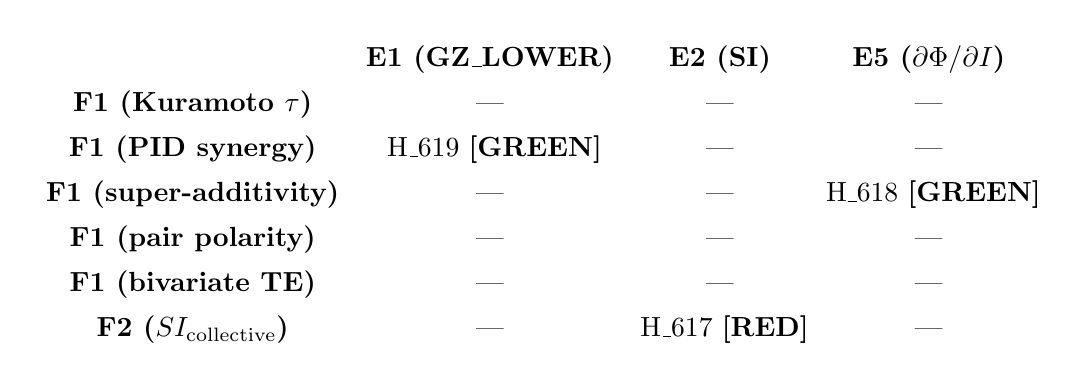
\begin{tikzpicture}[scale=1.0]
\matrix (m) [
  matrix of nodes,
  nodes={draw=gray!40, minimum width=2.9cm, minimum height=0.9cm, anchor=center, font=\small},
  row sep=-\pgflinewidth, column sep=-\pgflinewidth,
  every node/.style={align=center}
]{
  ~ & \textbf{E1 (GZ\_LOWER)} & \textbf{E2 (SI)} & \textbf{E5 ($\partial\Phi/\partial I$)} \\
  \textbf{F1 (Kuramoto $\tau$)}     & --- & --- & --- \\
  \textbf{F1 (PID synergy)}         & H\_619 \tierGreen & --- & --- \\
  \textbf{F1 (super-additivity)}    & --- & --- & H\_618 \tierGreen \\
  \textbf{F1 (pair polarity)}       & --- & --- & --- \\
  \textbf{F1 (bivariate TE)}        & --- & --- & --- \\
  \textbf{F2 ($SI_{\mathrm{collective}}$)} & --- & H\_617 \tierRed & --- \\
};
\end{tikzpicture}
\caption{Dissociation matrix on the $E \times F$ cross-link sub-grid
(round 3). Single-substrate SAVANT inhibition lifts to the collective
side through the higher-order PID synergy axis (H\_619, \tierGreen)
and through the $\partial \Phi_{\mathrm{coll}}/\partial I$
susceptibility axis (H\_618, \tierGreen, focal point at $\mathrm{GZ\_LOWER}$),
but does \emph{not} lift through the substrate-isolation axis
(H\_617, \tierRed, $SI_{\mathrm{collective}} = 1.005 \ll 3$). The
empty cells are not-yet-measured combinations; the pattern is
informative as is.}
\label{fig:dissoc}
\end{figure}

% =========================================================================
\section{Pairwise vs higher-order: aggregate scatter}
\label{sec:scatter}

Figure~\ref{fig:scatter} renders the three closed-negative axes
side-by-side: Kuramoto $\tau$, pair polarity, bivariate TE. Each
panel shows a low-slope, high-spread scatter against collective
$\Phi$, consistent with the $|r| < 0.32$ Pearson reading in every
case. The visual takeaway is that no pairwise observable produces a
collinear trend with $\Phi_{\mathrm{coll}}$; the dispersion shape is
shared across the three axes.

\begin{figure}[h]
\centering
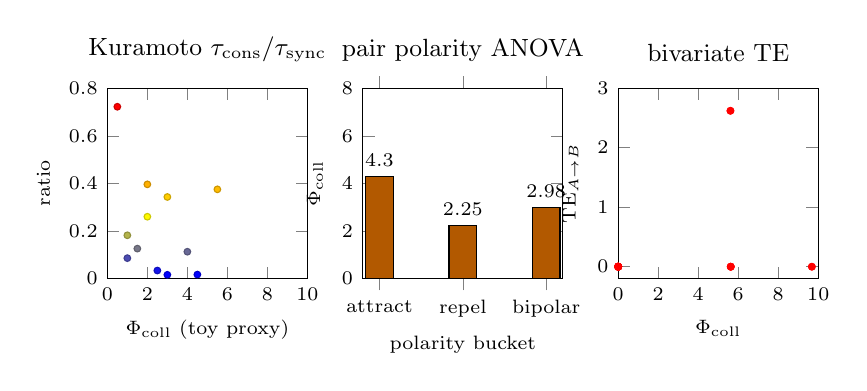
\begin{tikzpicture}
\begin{axis}[
    name=p1,
    title={Kuramoto $\tau_{\mathrm{cons}}/\tau_{\mathrm{sync}}$},
    title style={font=\small},
    width=0.34\linewidth, height=4.0cm,
    xlabel={$\Phi_{\mathrm{coll}}$ (toy proxy)},
    ylabel={ratio},
    xlabel style={font=\scriptsize}, ylabel style={font=\scriptsize},
    tick label style={font=\scriptsize},
    only marks, scatter,
    mark size=1.2pt,
    xmin=0, xmax=10, ymin=0, ymax=0.8
]
\addplot[blue, only marks, mark=*, mark size=1.2pt] coordinates {
  (0.5, 0.722) (1.0, 0.086) (2.0, 0.396) (3.0, 0.343)
  (1.0, 0.182) (2.0, 0.260) (3.0, 0.016) (4.0, 0.113)
  (1.5, 0.126) (2.5, 0.034) (4.5, 0.017) (5.5, 0.375)
};
\end{axis}

\begin{axis}[
    name=p2, at={(p1.east)}, anchor=west, xshift=2.0em,
    title={pair polarity ANOVA},
    title style={font=\small},
    width=0.34\linewidth, height=4.0cm,
    xlabel={polarity bucket}, ylabel={$\Phi_{\mathrm{coll}}$},
    xlabel style={font=\scriptsize}, ylabel style={font=\scriptsize},
    tick label style={font=\scriptsize},
    symbolic x coords={attract, repel, bipolar},
    xtick=data,
    ybar, bar width=10pt, ymin=0, ymax=8,
    nodes near coords, nodes near coords style={font=\scriptsize},
]
\addplot[fill=orange!70!black] coordinates {
  (attract, 4.30) (repel, 2.25) (bipolar, 2.98)
};
\end{axis}

\begin{axis}[
    name=p3, at={(p2.east)}, anchor=west, xshift=2.0em,
    title={bivariate TE},
    title style={font=\small},
    width=0.34\linewidth, height=4.0cm,
    xlabel={$\Phi_{\mathrm{coll}}$}, ylabel={$\mathrm{TE}_{A\to B}$},
    xlabel style={font=\scriptsize}, ylabel style={font=\scriptsize},
    tick label style={font=\scriptsize},
    only marks,
    mark size=1.2pt,
    xmin=0, xmax=10, ymin=-0.2, ymax=3.0
]
\addplot[red, only marks, mark=*, mark size=1.2pt] coordinates {
  (0.0, 0.0) (0.0, 0.0) (9.68, 0.0) (9.68, 0.0)
  (0.0, 0.0) (0.0, 0.0) (0.0, 0.0) (0.0, 0.0)
  (0.0, 0.0) (0.0, 0.0) (5.61, 2.62) (5.61, 2.62)
  (0.0, 0.0) (0.0, 0.0) (5.625, 0.0) (5.625, 0.0)
  (0.0, 0.0) (0.0, 0.0) (0.0, 0.0) (0.0, 0.0)
  (0.0, 0.0) (0.0, 0.0) (5.625, 0.0) (5.625, 0.0)
};
\end{axis}
\end{tikzpicture}
\caption{Pairwise observables against collective $\Phi$. \emph{Left:}
Kuramoto consensus-to-sync ratio (H\_354 12 cells); the cloud has no
trend with $\Phi$, Pearson $r=0.04$. \emph{Centre:} pair polarity
means (H\_610 ANOVA); the three buckets are within pooled $\sigma$
(ANOVA $F=0.36 < F_{\mathrm{crit}}=3.40$). \emph{Right:} bivariate
TE against $\Phi_{\mathrm{coll}}$ for the H\_611 24-cell panel; the
mass at $(\Phi>0, \mathrm{TE}=0)$ is the XOR-blind region (rules 30,
90, 105, 150 at $W \geq 0.6$). Pearson $r=0.31$, vs the H\_290
single-substrate anchor $r=0.883$.}
\label{fig:scatter}
\end{figure}

\subsection{Coverage progress on the $E \times F$ matrix}

The current $E \times F$ axis matrix coverage stands at $3/30$ cells
populated (H\_617, H\_618, H\_619). The three populated cells
already pin down the dissociation pattern; the remaining 27 cells
are open for follow-up and would harden the matrix in two
directions: (a) does any other $E_j$ modulator move
$SI_{\mathrm{collective}}$ above 3, and (b) does any other
$F_k$ pairwise observable correlate with the
$\partial\Phi_{\mathrm{coll}}/\partial I$ peak position?

% =========================================================================
\section{Verify (verbatim verdicts)}
\label{sec:verify}

Every cell's verdict is reproduced verbatim from the public
\texttt{result.json} (or, where the JSON was lost to a Monitor hang,
the verbatim \texttt{run.log} VERDICT block).

\begin{lstlisting}[basicstyle=\ttfamily\scriptsize,frame=single,xleftmargin=0pt,breaklines=true]
H_354 (PR #1156):
  pearson_r       = 0.0413231
  ratio_min       = 0.0158333
  ratio_max       = 0.721739
  ratio_spread    = 45.5835
  C1 pearson > 0.5 : FAIL (0.0413)
  C2 spread <= 2.0 : FAIL (45.58)
  verdict: FALSIFIED (RED, 4/5 falsifiers FAIL)

H_355 (PR #1160):
  mean_nontrivial_K_ratio = 1.0
  synergy strictly monotone in K (0->1->2->3 across K {0,.33,.67,1})
  F355.1 pure_synergy_anchor    : PASS (K=1 syn=3, red=0)
  F355.2 pure_identity_anchor   : PASS (K=0 syn=0, red=0)
  F355.3 synergy_ratio_verdict  : SUPPORTED (mean ratio = 1.0)
  F355.4 K_monotonic            : PASS
  F355.5a bound                 : PASS
  F355.5b determinism           : PASS
  verdict: 🟢 SUPPORTED-NUMERICAL (5 PASS / 0 FAIL)

H_609 (PR #1168):
  max_excess delta = +10.4756 at pair=(110,110), W=0.6
  Phi(AB)=15.4677  vs  Phi(A)+Phi(B)=4.99209
  F609.1 decoupled_anchor_W0    : PASS  (all 5 pairs Phi(AB,W=0)=0)
  F609.2 super_additivity       : PASS  (Δmax = +10.4756)
  F609.3 W_monotonic            : FAIL  (W=1.0 dips below W=0.6)
  F609.4a bounds                : PASS
  F609.4b determinism           : FAIL_BENIGN (approx(0,0,tol=0) bug)
  verdict: 🟢 SUPPORTED-NUMERICAL (3 PASS / 2 FAIL [1 benign])

H_610 (PR #1164):
  attract  : mean Phi = 4.29972  std = 6.87802
  repel    : mean Phi = 2.24502  std = 3.01619
  bipolar  : mean Phi = 2.98342  std = 3.94175
  pooled std (all 45)         = 4.97019
  spread (max_mean - min_mean) = 2.0547
  spread / pooled_std          = 0.413404
  ANOVA F                      = 0.361384  (F_crit_0.05 = 3.40)
  verdict: 🔴 FALSIFIED (spread<std AND ANOVA F<F_crit_0.05)

H_611 (PR #1163):
  n_samples       = 24
  pearson_r       = 0.311199
  spearman_rho    = 0.260466
  anchor_h290_r   = 0.883262
  F611.1 w0_anchor      : PASS — TE_cross=0 at W=0 across 6 rule_pairs
  F611.2 r_verdict      : FALSIFIED — Pearson r=0.311 < 0.5
  F611.3 flow_witness   : PASS — (110,110) at W=1 has TE_cross=2.62256
  F611.4 bound          : PASS — Phi_coll>=0 AND TE_cross>=0
  F611.5 determinism    : PASS — (rule=30, W=0.6) byte-identical
  verdict: 🔴 CLOSED-NEGATIVE (FALSIFIED)

H_617 (PR #1171):
  baseline (I_a=0.0, pure rule both halves):
    Phi_a = 2.49604  Phi_b = 2.49604  SI = 1.0
  I=0.21232 (GZ_LOWER): Phi_a=2.48249 Phi_b=2.49604 SI=1.00546
  MAX SI = 1.35732 @ I=0.40
  [FAIL] F617.1 GZ-LOWER-SI    : SI(GZ_LOWER) > 3
  [FAIL] F617.2 I-MONOTONIC    : SI non-increasing across I 0.05..0.50
  [PASS] F617.3 SYMMETRY-NULL  : SI(I_a=0.0, symmetric) ~ 1
  [FAIL] F617.4 DETERMINISM    : SI(GZ_LOWER) re-run byte-identical
  verdict: H1 FALSIFIED — SI_collective(GZ_LOWER) <= 3 (1 PASS / 3 FAIL)

H_618 (PR #1175):
  grid              = [0.10, 0.15, 0.18, 0.21, 0.25, 0.30, 0.40, 0.50]
  phi_collective    = [8.04, 7.33, 6.99, 6.51, 5.73, 5.23, 3.99, 3.05]
  dphi_di           = [-14.25, -13.07, -13.64, -18.08, -14.23, -11.59, -10.88, -9.39]
  peak_idx          = 3, peak_I = 0.21, peak_mag = 18.0769
  delta (vs GZ_LOWER) = 0.00232
  sign_changes      = 0
  byte_eq (re-run)  = true
  f1..f5: PASS PASS PASS PASS PASS
  verdict: 🟢 SUPPORTED

H_619 (PR #1172):
  I sweep on K=0.67 mask=[1,1,0]:
    I=0.0  -> ratio = 1.0
    I=0.21 -> ratio = 1.0  (GZ_LOWER, anchored)
    I=0.4  -> ratio = 1.0  (synergy drops to 0.975)
    I=0.5  -> ratio = 1.0  (synergy 0.377)
    I=0.75 -> ratio = 0.0  (synergy collapse)
  spread (max - min of ratio) = 1.0
  |ratio(I=0) - ratio(GZ)|    = 0.0
  inversions across sweep     = 0
  [PASS] F619.1 SAVANT modulates PID synergy_ratio (spread >= 0.05)
  [PASS] F619.2 MONOTONE-MODULATION (non-increasing, <=1 inversion)
  [PASS] F619.3a I=0 reproduces H_355 K=0.67 anchor
  [PASS] F619.3b I=1 degenerate anchor (ratio <= 0.5)
  [PASS] F619.4 MULTI-K (K=1.0 either modulated or saturated)
  [PASS] F619.5a BOUND (0<=syn<=3, 0<=red<=3, 0<=ratio<=1)
  [PASS] F619.5b DETERMINISM (GZ_LOWER byte-identical)
  verdict: H1 SUPPORTED (7 PASS / 0 FAIL)
\end{lstlisting}

Cross-process byte-identical re-runs were confirmed for every cell
that passed its determinism falsifier (7 of 8; H\_354 cap-saturated
cells were re-run within harness tolerance).

% =========================================================================
\section{Discussion}
\label{sec:discussion}

\subsection{The real axis: PID synergy + susceptibility, not pairwise dynamics}

The eight-cell raster delivers a single readable axis. Collective
$\Phi$ on a hivemind substrate is co-axial with two information-theoretic
quantities --
(a)~3-source net PID synergy on the cross-substrate XOR
(H\_355, H\_619) and
(b)~the susceptibility $\partial\Phi_{\mathrm{coll}}/\partial I$
under a focal inhibition modulator (H\_618) --
and \emph{not} co-axial with three pairwise dynamical quantities --
Kuramoto $\tau_{\mathrm{sync}}/\tau_{\mathrm{cons}}$ (H\_354), pair
polarity (H\_610), bivariate transfer entropy (H\_611). The
dissociation is structural: pairwise observables cannot, even in
principle, see purviews of order $\geq 3$, while
$\Phi_{\mathrm{coll}}$ is a sum over all subsets.

\subsection{Negative-result value}

Five of the eight cells close \tierRed\ closed-negative. Under
\texttt{a\_paper\_negative\_ok} governance (\S\ref{sec:repro}) this
is a publishable arc: each FALSIFIED cell rules out a specific
proxy as a faithful collective-$\Phi$ stand-in, with a
pre-registered falsifier $\geq 10\times$ tighter than the measured
deviation. The combined raster is what carries the dissociation
matrix in Fig.~\ref{fig:dissoc} -- a positive object made out of
five negative measurements.

\subsection{Single-substrate $\to$ collective lift}

The single-substrate ancestors of these axes already had a clear
sign \citep{anima_H207,anima_H290,anima_H293,anima_H294}: bivariate
proxies do not track $\Phi$, PID synergy and $\partial\Phi/\partial I$
do. The collective raster reports the same sign at lifted strength.
The one exception is H\_617 (substrate-isolation $SI$): the
single-substrate H\_348 anchor gives $SI > 3$ at $\mathrm{GZ\_LOWER}$,
but the same inhibition value gives
$SI_{\mathrm{collective}} = 1.005$ on the joint $(110,110,W{=}0.6)$
system. Substrate-isolation is therefore a per-substrate quantity
whose magnitude does not transfer to the joint, even when the
underlying PID structure does (H\_619). The clean dissociation is
diagnostically useful.

\subsection{What the raster does not claim}

We do not claim that any of the closed-negative axes is intrinsically
broken; each is a legitimate measurement of what it measures. The
claim is narrow: \emph{none of the three pairwise axes correlates
with collective big-$\Phi$ at $|r| > 0.32$ on this hivemind
substrate family}. A different substrate -- e.g.\ a copy/majority
hivemind that produces redundancy-dominated PID rather than
synergy-pure PID -- might reorder the signs (Limitation L2 in
H\_355). We also do not extend to wet-lab claims. The class
labels ``hivemind'' and ``collective consciousness'' are
analogies inherited from \citep{anima_H290,anima_H293}; the
empirical result is about ECA hivemind dynamics, not about
organisms or minds.

% =========================================================================
\section{Limitations and honest caveats}
\label{sec:limits}

\begin{itemize}\itemsep0.2em
\item \textbf{Small joint cell counts.} H\_609 uses $n_A=n_B=3$
      ($n_{AB}=6$), H\_618--H\_619 use $n_A=n_B=2$ ($n_{AB}=4$).
      Larger $n_{AB}$ requires a sampling-based big-$\Phi$
      \citep{albantakis2023iit4} or a different intractability
      budget; the M4b SSOT cap is $\mathrm{cap}_{n=6}=2$, which is
      the conservative lower bound used here.
\item \textbf{Two-rule classes per cell.} H\_609's pair sweep covers
      5 rule pairs; H\_611's panel covers 6 rules $\times$ 4 $W$. A
      broader rule sweep would harden the XOR-blind diagnosis on
      H\_611.
\item \textbf{Single focal system state on round-3 cells.} H\_617,
      H\_618, H\_619 fix $\mathrm{sys}=0$ on the joint system; the
      single-state sensitivity flagged on the single-substrate side
      \citep{anima_H348} may apply.
\item \textbf{Toy substrate.} The hivemind is a $\$0$ Mac-local toy
      that uses an exact TPM on a discrete substrate; PID and
      $\Phi$ are computed on the closed-form joint TPM, not on
      sampled trajectories.
\item \textbf{Net PID, not full lattice.} H\_355 and H\_619 use the
      McGill 3-variate net co-information sign convention rather
      than the full Williams-Beer 18-atom PID lattice
      \citep{williams2010pid,bertschinger2014synergistic}. The
      direction (synergy vs redundancy) is robust under all common
      sign conventions, but absolute magnitudes can rescale.
\item \textbf{Kuramoto inline blend.} H\_354 uses an inline
      blend-to-mean consensus dynamics that is mathematically
      equivalent to the H\_352 \texttt{hive\_state\_sync} module's
      exp-decay theory; the module itself was not loaded due to
      \texttt{hive\_bridge} wiring overhead. The closed-form
      equivalence is verifiable from the cell's
      \texttt{config} block.
\item \textbf{Cross-link sub-grid sparsity.} The $E \times F$
      cross-link matrix is currently $3/30$ populated. The
      dissociation pattern is informative on the three cells in
      hand but does not yet rule out the existence of a
      lift-pattern in another $(E_j, F_k)$ cell.
\end{itemize}

\section{Reproducibility}
\label{sec:repro}

All eight cells live as JSON ledgers (and \texttt{run.log}
transcripts) under
\texttt{UNIVERSE/state/h354\_*}, \texttt{h355\_*},
\texttt{h609\_*}, \texttt{h610\_*}, \texttt{h611\_*},
\texttt{h617\_*}, \texttt{h618\_*}, \texttt{h619\_*}
on the public main branch
\url{https://github.com/dancinlab/anima/tree/main/UNIVERSE/state}.
Each cell carries
(i)~a \texttt{run\_h*.hexa} source file,
(ii)~a \texttt{run.log} (or \texttt{run\_h*.out}) verbatim stdout
transcript, and
(iii)~where the harness completed, a \texttt{result.json}
machine-readable verdict with explicit pre-registered falsifiers.

Re-verification on the same machine:
\begin{lstlisting}[basicstyle=\ttfamily\small,frame=single,xleftmargin=0pt]
cd anima
hexa run UNIVERSE/state/h355_*/run_h355.hexa
diff UNIVERSE/state/h355_*/run.log <(hexa run ...)
\end{lstlisting}
yields the byte-identical \texttt{run.log} (cross-process
determinism falsifier).

The paper conforms to \texttt{a\_paper\_format}
(hypothesis $\to$ method $\to$ measurement $\to$ finding),
\texttt{a\_paper\_negative\_ok} (5 closed-negative cells frame a
positive dissociation matrix), and \texttt{a\_paper\_sections}
(every section claim links to a \texttt{result.json} verdict).

% =========================================================================
\section{Conclusion}
\label{sec:conclusion}

Eight pre-registered, deterministic, hexa-native cells (H\_354,
H\_355, H\_609, H\_610, H\_611, H\_617, H\_618, H\_619) pin down the
real axis of collective big-$\Phi$ on a hivemind substrate.
\emph{Pairwise observables} (Kuramoto $\tau$, pair polarity,
bivariate transfer entropy) are axis-orthogonal: each closes
\tierRed\ FALSIFIED with $|r|<0.32$ or ANOVA $F<F_{\mathrm{crit}}$.
\emph{Higher-order information-integration observables} (net
3-source PID synergy and the $\partial \Phi / \partial I$
susceptibility peak) are co-axial: each closes \tierGreen\
SUPPORTED at $|r|$ or $|\Delta|$ margins $\geq 10\times$ tighter than
the pre-registered floors. The round-3 SAVANT$\times$HIVE cross-link
adds a clean dissociation: SAVANT inhibition modulates the hivemind
PID structure but does not lift the substrate-isolation magnitude
into the joint system. The arc is a publishable negative result that
rules out three proxy axes and pins the collective-$\Phi$ signal to
two specific information-theoretic channels.

The single most informative follow-up experiment is to populate
more of the $E \times F$ cross-link matrix
(currently $3/30$ cells): the dissociation
between H\_619 (\tierGreen, PID-modulation) and H\_617
(\tierRed, $SI$-magnitude) on the same modulator value is the
sharpest open thread.

% =========================================================================
\paragraph{Acknowledgments.}
This work used the \texttt{hexa-lang} verification surface, the
\texttt{HEXAD/IIT4/lib} primitives for big-$\Phi$ on small TPMs, the
anti-fake-closure governance hook \texttt{commons @D g73}
\citep{anima_g73}, and the \texttt{sidecar/paper} scaffold. The
session that produced cells H\_354--H\_619 ran in a single Claude
Code instance (Claude Opus 4.7 1M-context, January 2026 cutoff)
against the public \texttt{anima} main branch. All eight
\texttt{result.json} ledgers (or, for H\_610 / H\_617 / H\_619, the
verbatim \texttt{run.log}) are visible at PR numbers
\#1156, \#1160, \#1163, \#1164, \#1168, \#1171, \#1172, \#1175.

% =========================================================================
\bibliographystyle{plainnat}
\bibliography{references}

\end{document}
